\documentclass{article}

\usepackage[utf8]{inputenc}
% \usepackage[utf8]{inputenc}
\usepackage{multicol}
\usepackage{dcolumn}
\usepackage[a4paper,top=3cm,bottom=3cm,left=1.5cm,right=1.5cm,marginparwidth=1.75cm]{geometry}
\usepackage{multicol}
\setlength{\columnsep}{0.5cm}
\usepackage{multirow}
\usepackage{amsmath}
\usepackage{graphicx}
\usepackage{hyperref}
\hypersetup{colorlinks=true,linkcolor=blue,filecolor=magenta,urlcolor=cyan,}
\usepackage{amsfonts}
\usepackage{mathtools}
\usepackage{lipsum}
\usepackage{float}
\usepackage{layout}
\usepackage{bm}

\usepackage{listings}
\usepackage{xcolor}
\definecolor{codegreen}{rgb}{0,0.6,0}
\definecolor{codegray}{rgb}{0.5,0.5,0.5}
\definecolor{codepurple}{rgb}{0.58,0,0.82}
\definecolor{backcolour}{rgb}{0.95,0.95,0.92}
\lstdefinestyle{mystyle}{
    backgroundcolor=\color{backcolour},
    commentstyle=\color{codegreen},
    keywordstyle=\color{blue},
    numberstyle=\tiny\color{codegray},
    stringstyle=\color{codepurple},
    basicstyle=\ttfamily\footnotesize,
    breakatwhitespace=false,
    breaklines=true,
    captionpos=b,
    keepspaces=true,
    numbers=left,
    numbersep=5pt,
    showspaces=false,
    showstringspaces=false,
    showtabs=false,
    tabsize=2
}
\lstset{style=mystyle}





\begin{document}










%TitlePage%TitlePage%TitlePage%TitlePage%TitlePage%TitlePage%TitlePage%TitlePage%TitlePage%TitlePage%TitlePage%TitlePage%TitlePage
\thispagestyle{empty}
\baselineskip25pt
\begin{center}
{\Large {\textbf{EXPERIMENTS WITH LOCK-IN-AMPLIFIER USING EXPEYES (Calibration, Low Resistance and CV profiling)}}}\\
\end{center}

\vfill
\baselineskip15pt
\begin{center}
{\em Open Lab Report Submitted} \\
in Partial Fulfilment of the Requirements \\
for the course \
\vskip .30\baselineskip
{\large{\bf P442-Integrated Laboratory-II}}
\end{center}
\baselineskip25pt

\vfill
\begin{center} {\bf {\em by}} \\
{\large{\bf ANANTHA PADMANABHAN M NAIR}} \\
Course Instructors:\\
\textbf{Dr. Ashok Mohapatra\\
Dr. Gunda Santosh Babu}
\end{center}

\vfill
\begin{center}
\begin{figure}[h!]
\centering

\includegraphics[scale=0.2]{Images/logo1.jpg}
\end{figure}
 {\bf {\em to the }} \\
{\bf {\large School of Physical Sciences}} \\
{\bf {\large National Institute of Science Education and Research}} \\
{\bf Bhubaneswar} \\
{\bf \today} 
\end{center}
%TitlePage%TitlePage%TitlePage%TitlePage%TitlePage%TitlePage%TitlePage%TitlePage%TitlePage%TitlePage%TitlePage%TitlePage%TitlePage%










%Content Table Page%Content Table Page%Content Table Page%Content Table Page%Content Table Page%Content Table Page
\pagenumbering{roman}
\newpage
\newgeometry{top=2.5cm,bottom=2.5cm,left=3.5cm,right=3.5cm}
\begin{center}
 \tableofcontents  
 \newpage
 \listoffigures
 \listoftables 
\end{center}
\restoregeometry
%Content Table Page%Content Table Page%Content Table Page%Content Table Page%Content Table Page%Content Table Page



\newpage
\begin{center}
    \large{\textbf{EXPERIMENTS WITH LOCK-IN-AMPLIFIER USING EXPEYES\\ (Calibration, Low Resistance and CV profiling)}}
\end{center}
\begin{abstract}
    This experiment primarily centres on constructing a Lock-in amplifier using ExpEYES/SeeLAB, validating its functionality, and subsequently conducting various experiments employing the built apparatus. These experiments encompass calibration, low resistance measurement, and CV profiling of both monocrystalline and polycrystalline solar cells. The obtained results demonstrated close conformity with actual data. Furthermore, given the affordability and accessibility of the components utilized, this cost-effective approach to lock-in detection proves to be particularly suitable for instructional laboratories 
\end{abstract}
\begin{multicols}{2}
\pagenumbering{arabic}



\section{Introduction}

A flexible open-source hardware and software framework called ExpEYES, which stands for "Experiments for Young Engineers and Scientists," is intended for use in physics, electronics, biology, and chemistry investigations. ExpEYES, created by the Inter-University Accelerator Centre in India, offers a practical and affordable approach to science teaching and experimentation. The lock-in amplifier operates on the basis of phase-sensitive detection, in which the target signal is efficiently isolated from noise by modulating it at a known frequency and then demodulating it at the same frequency. 


%%%%%%%%%%%%%%%%%%%%%%%%%%%%%%%%%%%%%%%%%%%%%%%%%%%%%%%%%%%%%%%%%%%%%%%%%%%%%%%%%%%%%%%%%%%%%%%%%%%%%%%%%%%%%%%%%%%%%%%%%%%%%%%%%%%%%%%%%%%%%%%%%%%%%%%%%%
\section{\label{theory}Theory}


A lock-in amplifier serves the purpose of detecting minute voltages amid noisy environments. This is accomplished through phase-sensitive detection, a technique employed by commercially accessible lock-in amplifiers. In order to amplify the signal from the noise, we must know the frequency of the signal that has to be separated. 


In the lock in amplifier, we use a reference signal which has the same frequency as that of the noisy signal. We multiply the signal with the reference as well as a reference shifted by a phase of $\pi/2$ and then we put a low pass filer to get the DC components and hence we get the amplitude of the corresponding signal. Let's see how that's implemented.



Let the signal that we want to measure be a sine wave of frequency $\omega_{sig}$ and amplitude $V_{sig}$. Consider this is the signal that is embedded in the noise. This can be represented by:


\begin{equation}
    V_{sig}(t) = V_{sig} \sin(\omega_{sig}t + \phi)
\end{equation}

Let the reference signals be:
\begin{eqnarray}
    V_{ref}^0(t) = V_{ref} \sin(\omega_{ref}t)\\
    V_{ref}^{90}(t) = V_{ref} \cos(\omega_{ref}t)
\end{eqnarray}

Multiplying equations (2) and (3) with (1), we get:

\begin{eqnarray}
    V_{sig}(t) V_{ref}^0(t) = V_{sig} V_{ref} \sin(\omega_{sig}t + \phi) \sin(\omega_{ref}t)\\
    V_{sig}(t) V_{ref}^{90}(t) = V_{sig} V_{ref} \sin(\omega_{sig}t + \phi) \cos(\omega_{ref}t)
\end{eqnarray}


Let's call the former $V^0(t)$, the in-phase component and the latter one $V^90 (t)$, as the quadrature component. So, after using trigonometric identities and setting $\omega_{ref} = \omega_{sig} $ we get these components as: 

\begin{eqnarray}
    V^0(t) = \frac{V_{sig} V_{ref}}{2} \cos(\phi) + \frac{V_{sig} V_{ref}}{2} \cos(2\omega_{ref}t + \phi)\\
    V^{90}(t) = \frac{V_{sig} V_{ref}}{2} \sin(\phi) + \frac{V_{sig} V_{ref}}{2} \sin(2\omega_{ref}t + \phi)
\end{eqnarray}

Now if we set $V_{ref} = 2V$, we get the components as:
\begin{eqnarray}
    V^0(t) = V_{sig} (\cos(\phi) +  \cos(2\omega_{ref}t + \phi))\\
    V^{90}(t) = V_{sig}(\sin(\phi) + \sin(2\omega_{ref}t + \phi))
\end{eqnarray}

Now we can perform a low pass filter to get the DC components of each of these voltages which gives us the amplitude of the input signal.

The Low pass filtering is done by taking an FFT or Fast Fourier Transform of the in-phase and the Quadrature signals. Thus, by eliminating the other frequencies, we will get the required Amplitude of the input signal. 

Lets assume that after we take the FFT of the in-phase and the quadrature signals, we get the DC components as $V^0$ and $V^{90}$ respectively. Then
we can now clearly see that the magnitude of the amplitude is given by the following equation (after eliminating the higher frequency components):
\begin{equation}
    V_{sig} = \sqrt{{V^0}^2 + {V^{90}}^2}
\end{equation}

%%%%%%%%%%%%%%%%%%%%%%%%%%%%%%%%%%%%%%%%%%%%%%%%%%%%%%%%%%%%%%%%%%%%%%%%%%%%%

\subsection{Fast Fourier Transform}


The Fast Fourier Transform (FFT) is a powerful mathematical algorithm used to efficiently compute the discrete Fourier transform (DFT) and its inverse. By converting a signal from its time domain representation to its frequency domain representation, the FFT enables the analysis of signal components at different frequencies. This process helps in identifying dominant frequencies, filtering out noise, and extracting useful information from complex signals.



For our experiment, the Voltage values and the corresponding time values are stored in an array. The FFT of the array is then taken and plotted in the Frequency domain. As we know the Fourier transform of sine and cosine functions are delta functions. Since in the FFT, unlike the analytical Fourier transform, we will not get an infinity at the specific frequency in which the delta function is infinity. The height of the peak is calculated from the computing algorithm to be $V_{sig} \times \text{"The Length of the array"}$ . So, by dividing the peak value by the array length, we will get the $V_{sig}$.  


Now since we are taking the FFT we now have the real and imaginary part. This is for each of the in phase and quadrature signals. So, the amplitude of the signal $V_{sig}$ is given by:
\begin{equation}
    V_{sig} = \sqrt{{V^0}^2 + {V^{90}}^2}
\end{equation}

Where the $V^0$ and $V^{90}$ is obtained by dividing the peaks by the array length of the respective $V^0 (t)$  and $V^{90} (t)$



%%%%%%%%%%%%%%%%%%%%%%%%%%%%%%%%%%%%%%%%%%%%%%%%%%%%%%%%%%%%%%%%%%%%%%%%%%%%%
\subsection{Calibration of the LIA}
The Lock in amplifier is calibrated using a known signal from the function generator. A plot of the $V_{in}$  vs $V_{out}$ is made where $V_{in}$ is the input signal and the output signal is $V_{out}$. We can use either the peak-to-peak value of the voltage or the RMS value. The slope of the plot gives us the amplification factor of the Lock in amplifier. The calibration is mainly done when an external amplifier (Using IC741 or TL083) is connected before the LIA. This may be required if the input voltage is very low, the SEELab or ExpEYES may not be able to measure it properly. So, an amplification along with the calibration is required for the smooth working of the Lock in amplifier. From the slope of the Calibration curve, we can calculate the amplification factor $\alpha$ $(slope= \alpha)$.
%%%%%%%%%%%%%%%%%%%%%%%%%%%%%%%%%%%%%%%%%%%%%%%%%%%%%%%%%%%%%%%%%%%%%%%%%%%%%
\subsection{Measurement of Low Resistance}
We can measure the low resistance using the Lock in amplifier. The circuit diagram for this measurement is shown in the Figure-\ref{circuit_LR}. 



\begin{figure}[H]
    \centering
    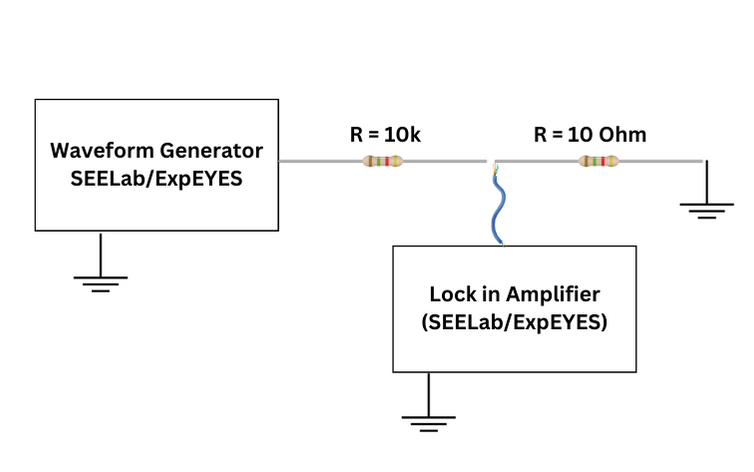
\includegraphics[width=\columnwidth]{Images/circuit_LR.png}
    \caption{Circuit Diagram for the Measurement of Low Resistance}
    \label{circuit_LR}
\end{figure}

In the figure, we set the resistance R to be much greater than the small resistance r. The total current through the circuit is given by:
\begin{equation}
    I = \frac{V}{R+r}
\end{equation}
Since $R>>r$, we can write $I=V/R$. As the resistances are connected in series, the current through them will be the same. So,
\begin{equation}
    \frac{V_R}{R} = \frac{V_r}{r} = \frac{V}{R}
\end{equation}


Also, we have the amplification factor $\alpha$, which was obtained from the calibration. Then $V_{out}=V_r \times \alpha$. So, we get:
\begin{equation}
    r = \frac{RV_{out}}{\alpha V}
    \label{LR_eqn}
\end{equation}
So by measuring the $V_{out}$ using the LIA, we can measure the low resistance r.



\subsection{C-V Profiling of Solar Cell}

Lock in Amplifier can also be used in the C-V-Profiling of not only the solar cell but also for Schottky Diodes, MOSFETS, etc. In Our case, we will be restricting ourselves to the case of Solar Cell only. We will be doing the profiling for the Monocrystalline as well as Polycrystalline solar cell.  The circuit Diagram for the same is shown below in Figure \ref{circuit_1_CV}.

\begin{figure}[H]
    \centering
    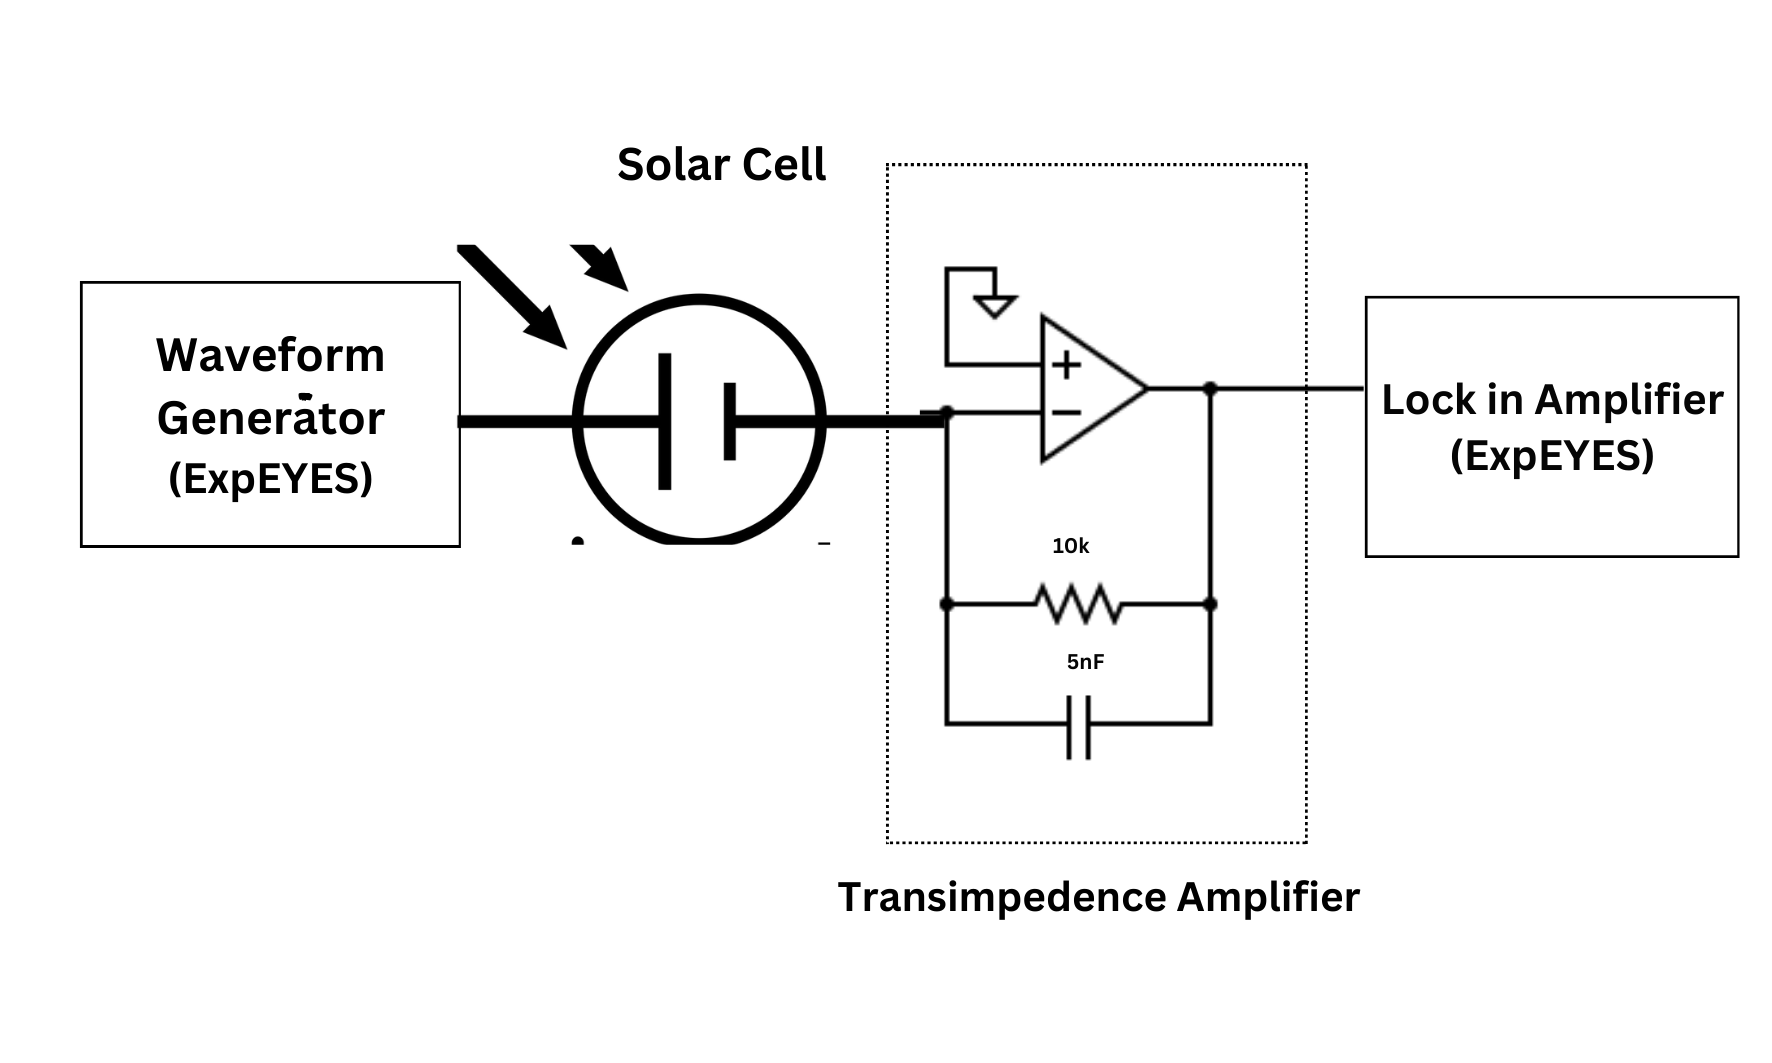
\includegraphics[width=\columnwidth]{Images/CV_1.png}
    \caption{Circuit Diagram CV Profiling of Solar Cell}
    \label{circuit_1_CV}
\end{figure}



For the solar cell, if we apply a reverse bias voltage $-V_R$, the net potential at the depletion region will become:
\begin{equation}
    -V_0 = -V_R + V_{bi}
\end{equation}



Where $V_{bi}$ is the built in potential of the silicon. Let the total charge on the surface be $-Q$. The depletion region will spread to a width $W$.as a result of semiconductor conduction electrons moving away from the interface. When the semiconductor reaches the depletion area, the electric field is zero and the semiconductor becomes neutral, negating the impact of $-Q$. $W$ is the screening length, and this effect is known as dielectric screening.


Firstly, for simplicity's sake, we'll assume a uniform doping density, where each dopant atom has a single charge $+e$, or $\rho(x) = \rho$ (a constant). By symmetry, we can infer that the electric field $\vec{E}$ in the depletion area points in the (negative) x-direction if the cross-sectional dimensions of the Depletion region are significantly larger than $W$. Then, using the rectangular Gaussian surface around the depletion region with one of its end caps in the neutral bulk region (where $\vec{E} = $0) and the other end cap located a distance x from the depletion region of n-p interface, The Gauss Law gives:
\begin{equation}
    \epsilon E A = \frac{+e \rho A \times (W-x)}{\epsilon_0}
\end{equation}


Where A is the area of the solar cell depletion region, and$\epsilon$ is the dielectric constant of the solar cell depletion region. Now to calculate the electric potential as a function of x, we impose
the boundary condition:
\begin{eqnarray}
    V(0) = -(V_R + V_{bi}) \\
    V(W) = 0
\end{eqnarray}


now we have:

\begin{eqnarray}
    V(W) - V(0) = \int_{0}^{W}  \vec{E} \cdot d\vec{x} \\
    \text{where } \vec{E} = \frac{+e \rho(W-x)}{\epsilon \epsilon_0} \hat{x}
\end{eqnarray}

on solving the above equation we get:
\begin{equation}
    V_R + V_{bi} = \frac{e \rho W^2}{2 \epsilon \epsilon_0}
    \label{vrvbi}
\end{equation}



on solving for the depletion width $W$ we get:
\begin{equation}
    W = \sqrt{\frac{2 \epsilon \epsilon_0 (V_R + V_{bi})}{e \rho}}
    \label{W}
\end{equation}


Now if we increase the reverse bias voltage by $dV_R$, 
the depletion width will
increase by $dW$ and the charge on the surface will increase 
by $dQ$. The extra space charge
and the $dQ$ is related as $dQ = e\rho A dW$. So, 
differentiating the equation-\ref{vrvbi} we get:

\begin{equation}
    dV_R = \frac{e \rho A WdW}{\epsilon \epsilon_0} = \frac{WdQ}{\epsilon \epsilon_0 A}
\end{equation}

Now we can relate the capacitance to the doping density as:

\begin{equation}
    C = \frac{dQ}{dV_R} = \frac{\epsilon \epsilon_0 A}{W}
\end{equation}

Now using the equation-\ref{W} we can write the capacitance as:


\begin{equation}
    \frac{1}{C^2} = \frac{2}{A^2e\epsilon \epsilon_0 \rho} (V_R + V_{bi})
    \label{CV_eqn}
\end{equation}

So for a Solar cell depletion region, the plot of $1/C^2$ vs $V_R$ is a straight  line with slope $\frac{2}{A^2e\epsilon \epsilon_0 \rho}$ and  intercept $V_{bi}$ from where we can calculate the doping density and the built  in potential.\cite{reynolds2014capacitance}


\subsubsection{Autophasing}

There could be more stray sources of capacitance in the 
circuit in addition to the capacitance of interest. We must 
remove unnecessary capacitance in order to improve the 
accuracy of our measurements. The method employed for 
this is autophasing. This technique's primary idea is to 
take a sort of dot product and project the device's 
capacitance onto an ideal capacitor. 


Here, we replace our device with an ideal 
calibration capacitor of known value $(C_0)$.
The in-phase ($V_{x0}$) and the quadrature components ($V_{y0}$) of the 
voltage obtained from this capacitor are
measured through lock-in detection and are 
noted for all the biasing voltages. Using
these values, the capacitance of the 
device (C) can be calculated as: 


\begin{equation}
    C = \frac{V_{0x}V_x + V_{0y}V_y }{V_{0x}^2 + V_{0y}^2} \times C_{0}
\end{equation}
where $V_x$ and $V_y$ are the in-phase and quadrature components obtained from the device.


%%%%%%%%%%%%%%%%%%%%%%%%%%%%%%%%%%%%%%%%%%%%%%%%%%%%%%%%%%%%%%%%%%%%%%%%%%%%%
%%%%%%%%%%%%%%%%%%%%%%%%%%%%%%%%%%%%%%%%%%%%%%%%%%%%%%%%%%%%%%%%%%%%%%%%%%%%%
\section{Experimental Setup and Procedure }


The Setup of the Experiment mainly involves the use of the python library of the ExpEYES/SEELab called the eyes17 library in python. The signal required for the processing is collected by the A1/A2 port of the ExpEYES. Both of the reference signals for the LIA are generated (it is because we assume that we already know the frequency of the signal that we need) within the software itself using the NumPy library.


\subsection{Building the Lock-in Amplifier}

The first step is to import the python library eyes17. In order to access the device, we need the library. This is shown in the listing-\ref{importing}


\begin{lstlisting}[language=Python, caption=importing the libraries-\cite{harris2020array}-\cite{2020SciPy-NMeth}-\cite{Hunter:2007}-\cite{csparkresearch},label=importing]
    import numpy as np
    import math as m
    from scipy.fft import fft, ifft,fftfreq
    import eyes17.eyes
    p=eyes17.eyes.open()
    import time as tim    
\end{lstlisting}


For simplicity, we will create the Lock in amplifier as a python function. As discussed in the theory the signal and the references are multiplied and an FFT is taken. The FFT is taken from the SciPy library. And all the plots are made in Matplotlib. As the signal is collected in arrays of voltage and time values, our function will have to take the arguments as a list of voltage and time. Also, one of the other arguments is the frequency. It is important to note that the units of the time which should be in seconds before passing it to the LIA function. In the upcoming sections. The whole list has been divided by a factor of 1000 in order to maintain clarity in the units. The function is shown in the Listing-\ref{LIAfunc}.


\begin{lstlisting}[language=Python, caption=Defining the Lock-In-Amplifier Function,label=LIAfunc]
def LIA(V_in,t_in,f):
    V_in_sin=[]         
    V_in_cos=[]                      
    for i in range(len(V_in)):      
        V_in_sin.append(V_in[i]*2*np.sin(2*np.pi*f*t_in[i]))
        V_in_cos.append(V_in[i]*2*np.cos(2*np.pi*f*t_in[i]))
    V_out_sin_fft=fft(V_in_sin)
    V_out_cos_fft=fft(V_in_cos)
    V_out= np.sqrt((V_out_sin_fft[0].real/len(V_out_sin_fft))**+(V_out_cos_fft[0].real/len(V_out_cos_fft))**2)
    return V_out
\end{lstlisting}


The algorithm is exactly the same as that mentioned in the theory section. The outputs of the function LIA are "$V_{out}$" as we can see in the code, is the amplitude of the signal with frequency f present in the noisy signal. For the CV profiling the function has been modified to return the in phase and the quadrature components that is required for the autophasing as shown in the listing-\ref{LIA_CV_code}.

\begin{lstlisting}[language=Python, caption=Modified function for CV-Profiling,label=LIA_CV_code]
V_out_sin_fft=fft(V_in_sin)
Vx=V_out_sin_fft[0].real/len(V_out_sin_fft)
V_out_cos_fft=fft(V_in_cos)
Vy=V_out_cos_fft[0].real/len(V_out_cos_fft)
return Vx,Vy
\end{lstlisting}


The complete code and calculations for this experiment can be accessed in our \href{https://github.com/ananthapadmanabhan18/Lock_in_Amplifier_with_ExpEyes.git}{GitHub repository}.

The signals are taken as the inputs using the capture1 function in the eyes17 library by the following method:

\begin{lstlisting}[language=Python]
t,v = p.capture1(stri,8192,2)
\end{lstlisting}
The 8192 is the total number of samples that is to be measured in a single run of the above line and 2 is the time gap between each sample whose units is in microseconds. The time obtained above is in milliseconds which we have to convert to seconds before feeding it to the LIA.

The value of number of samples is chosen as a power of 2 (Maximum capacity for the device is 10000 samples in one run) so that the FFT can be taken easily. The time gap is chosen as 2 microseconds so that the signal is sampled at a good rate of 50 MSPS.

%%%%%%%%%%%%%%%%%%%%%%%%%%%%%%%%%%%%%%%%%%%%%%%%%%%%%%%%%%%%%%%%%%%%%%%%%%%%%
\subsection{Procedure}

The procedure mainly includes the building of the external circuit. The output from the WG of the SEELab is very restricted, that is it can only give out 80mV, 1V or 3V depending on the arguments of the following command:
\begin{lstlisting}[language=Python]
p.set_sine_amp(2)
p.set_sine(f)    
\end{lstlisting}

Where in the former line, one can set it as 0 for 80mV, 1 for 1V and 2 for 3V. Since we require a continuous variation of the sinusoidal potential, we will be using a potentiometer to divide the voltage and get the required voltage amplitude. 

\subsubsection{Calibration}
For the Calibration the output from the potentiometer is directly given to the IC741 with $100k\Omega$ feedback resistor and input resistance of $1k\Omega$ which together should give rise to an amplification of $100\times$. The software amplification been set to one for the sake of simplicity. For the calibration $R_f=100k\Omega$ is used as the feedback resistor in the inverting amplifier before LIA

\subsubsection{Measurement of Low Resistance}
For this part the, the circuit is the same as shown in Figure-\ref{circuit_LR}. The input of the potentiometer is given to the WG and the output to the high resistance R. the voltage across the small resistance r is measured using the built LIA. The resistances used are $R=10000\Omega$.


\subsubsection{C-V Profiling of Solar Cell}

The circuit for the CV profiling is shown in the Figure-\ref{circuit_1_CV}. Here we have built an adder circuit using the IC741 in order to add the DC voltage and a small DC signal. The DC signal is generated from the pv1 of the ExpEYES and the sine wave is generated from the WG.

Since, we want small perturbations with the DC voltage we need to add these signals together. So, the modified circuit for the CV profiling is shown in Figure \ref{circuit_2_CV}.


\begin{figure*}%[HT]
    \centering
    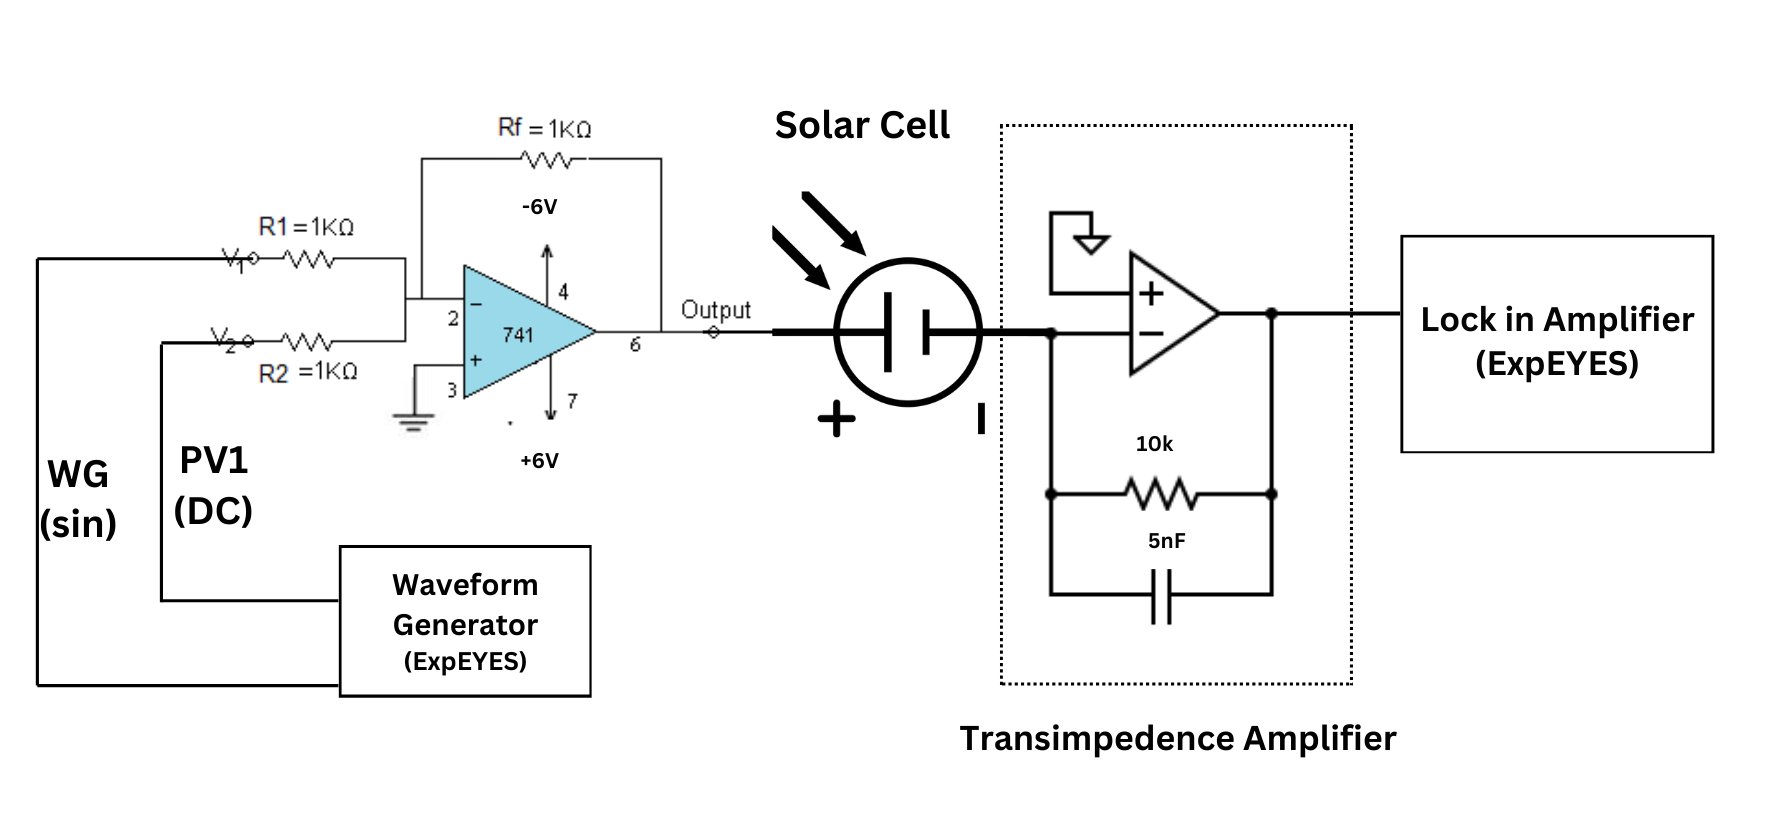
\includegraphics[width=2\columnwidth]{Images/CV_2.png}
    \caption{Modified Circuit Diagram CV Profiling of Solar Cell}
    \label{circuit_2_CV}
\end{figure*}


The resistances of the adder circuit are set in such a way that the net gain through the adder is 1. Unlike the Calibration the feedback resistance used in the transimpedance amplifier is 10k. and a 5nF capacitor is used. The calibration capacitor has a value of 5.56nF. which is used for further calculations. All this is done and it is made sure that the solar cell is reverse biased. In the circuit show above, there is a potentiometer in between WG and the adder circuit. For simplicity, it's not shown in the circuit.

The algorithm for the collection of data is that the $PV1$ Is varied in a loop and corresponding $V_x$  and $V_y$ are written to a text file, 1st with the calibration capacitor and then with the solar cell. The code for this is given below in listing \ref{CV_code}. Then the collected data is then used for further analysis

\begin{lstlisting}[language=Python, caption=Collecting the data as arrays for the CV-Profiling\cite{python},label=CV_code]
vset =[0.2,0.3,0.4,0.5,0.6,0.7,0.8,
        0.9,1.0,1.1,1.2,1.3,1.4,
        1.5,1.6,1.7,1.8,1.9,2,2.1]
j=0
for i in vset:
    p.set_pv1(i)
    tim.sleep(3)
    t,v=collect_signal('A1',N_sample,N_div,f)
    tim.sleep(3)
    Vx,Vy=LIA(v,t/1000,f)
    print(str(vset[j])+'\t'+str(Vx)+'\t'+str(Vy))
    with open('Data\\SS.txt','a') as file1:
        file1.write(str(vset[j])+'\t'+str(Vx)+'\t'+str(Vy)+'\n')
    j=j+1
\end{lstlisting}



The setup of the Cv-Profiling Experiment is shown in the Figure-\ref{CV_setup}.
\begin{figure}[H]
    \centering
    \includegraphics[width=0.6\columnwidth]{Images/CV_setup.jpg}
    \caption{Setup for the CV Profiling of Solar Cell (connected to calibration capacitor)}
    \label{CV_setup}
\end{figure}




%%%%%%%%%%%%%%%%%%%%%%%%%%%%%%%%%%%%%%%%%%%%%%%%%%%%%%%%%%%%%%%%%%%%%%%%%%%%%
\section{Observations and Data}

\subsection{Verification of working of the Lock in Amplifier}

The functioning of the Lock in amplifier was verified by using a known signal from generated in the python library with noise. The input signal and output were measured and plotted so as to verify the working of the LIA. The plot is shown in the Figure-\ref{LIA_verify}. Here the amplification is set to 10x virtually.

\begin{figure}[H]
    \centering
    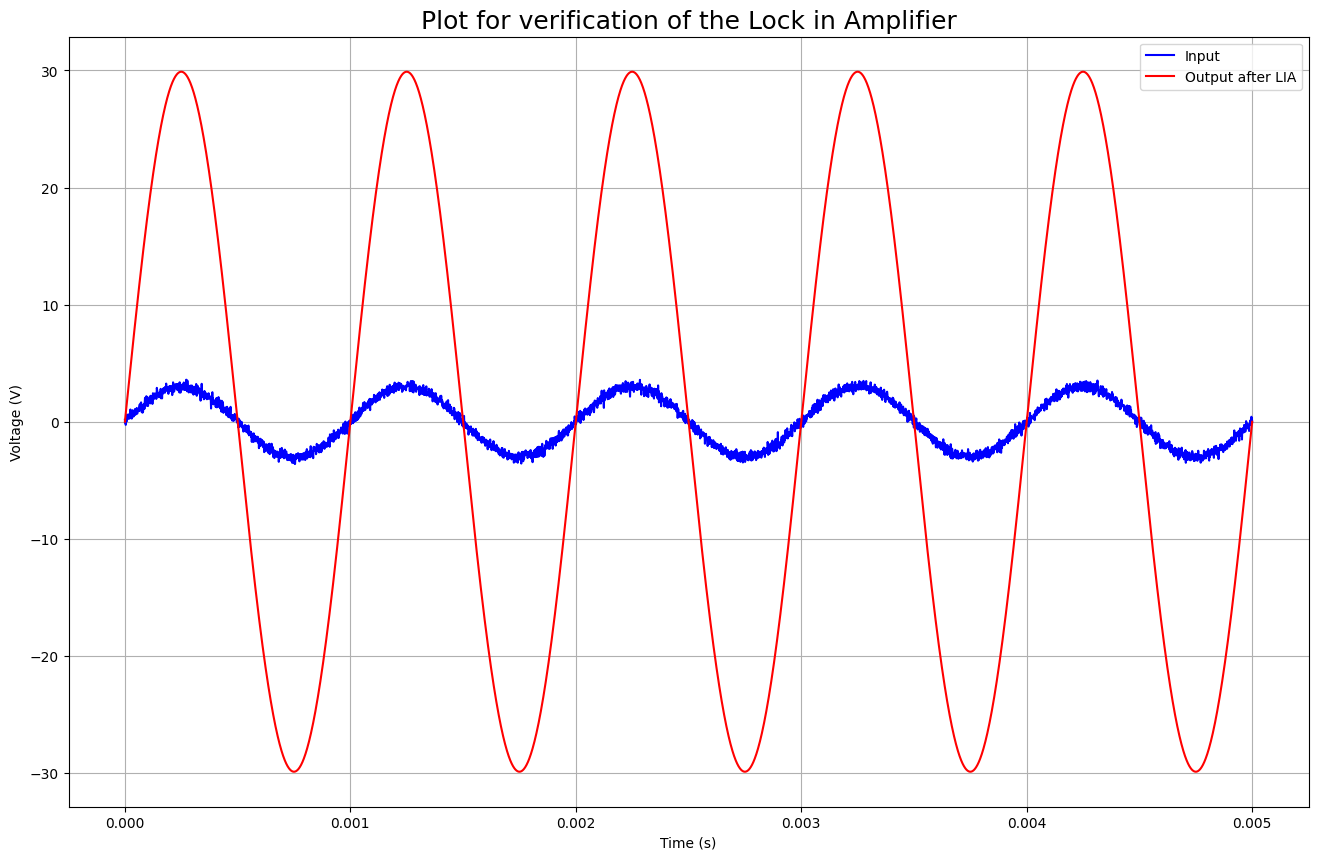
\includegraphics[width=\columnwidth]{Images/LIA_verify.png}
    \caption{Plot for verification of the working of the Lock in Amplifier function}
    \label{LIA_verify}
\end{figure}


Now a real signal from the WG of the SEELab is given to the A1 and the output is measured. The plot is shown in the Figure-\ref{LIA_verify_real}. Here the amplification is set back to unity.


\begin{figure}[H]
    \centering
    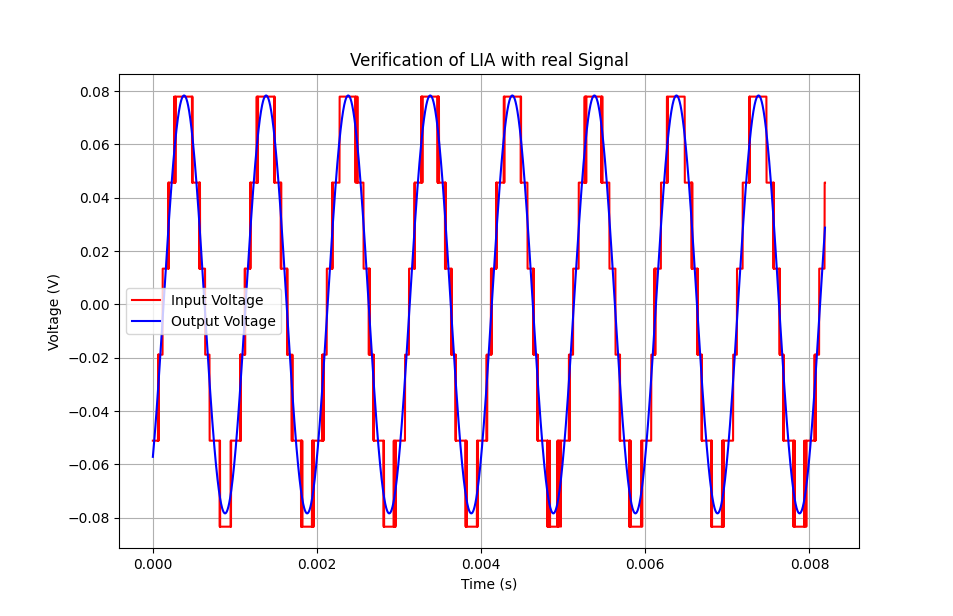
\includegraphics[width=\columnwidth]{Images/LIA_verify_real.png}
    \caption{Plot for verification of the working of the Lock in Amplifier function with a real signal from SEELab}
    \label{LIA_verify_real}
\end{figure}


The input signal and the reference signals had a phase difference of $\phi$. Since we are now obtaining the $V_x$ and $V_y$, this phase was removed following the amplification. The following formula is used to do this:
\begin{eqnarray}
    \phi  = \tan{^{-1}}{\frac{V_y}{V_x}}
\end{eqnarray}

This phase is added to the output signal so as to match with the input signal.





\subsection{Data for Calibration}

Data for the calibration is shown in the Table-\ref{CAL_data_table}.The data contains the input voltage, output voltage (both in RMS) for different frequencies of 500Hz, 1000Hz, and 2000Hz.


\begin{table*}
    \centering
    \resizebox{2\columnwidth}{!}{%
    \begin{tabular}{|c|cc|cc|cc|}
    \hline
    \multirow{2}{*}{\textbf{Sl   No}} & \multicolumn{2}{c|}{\textbf{500Hz}}                                 & \multicolumn{2}{c|}{\textbf{1000Hz}}                                & \multicolumn{2}{c|}{\textbf{2000Hz}}                                \\ \cline{2-7} 
                                      & \multicolumn{1}{c|}{\textbf{$V_{in}$ (V)}} & \textbf{$V_{out}$ (V)} & \multicolumn{1}{c|}{\textbf{$V_{in}$ (V)}} & \textbf{$V_{out}$ (V)} & \multicolumn{1}{c|}{\textbf{$V_{in}$ (V)}} & \textbf{$V_{out}$ (V)} \\ \hline
    1                                 & \multicolumn{1}{c|}{0.017182018}           & 1.203372531            & \multicolumn{1}{c|}{0.015671727}           & 1.149396809            & \multicolumn{1}{c|}{0.013987165}           & 1.047709881            \\ \hline
    2                                 & \multicolumn{1}{c|}{0.023065578}           & 1.492325673            & \multicolumn{1}{c|}{0.023028788}           & 1.528740499            & \multicolumn{1}{c|}{0.023391511}           & 1.479491873            \\ \hline
    3                                 & \multicolumn{1}{c|}{0.025554896}           & 1.978069124            & \multicolumn{1}{c|}{0.025688889}           & 2.04770376             & \multicolumn{1}{c|}{0.025175565}           & 1.828756137            \\ \hline
    4                                 & \multicolumn{1}{c|}{0.026813747}           & 2.387335743            & \multicolumn{1}{c|}{0.027003734}           & 2.641769499            & \multicolumn{1}{c|}{0.026062813}           & 2.016311599            \\ \hline
    5                                 & \multicolumn{1}{c|}{0.027089012}           & 2.636136896            & \multicolumn{1}{c|}{0.03309075}            & 3.039432545            & \multicolumn{1}{c|}{0.027024287}           & 2.475542671            \\ \hline
    6                                 & \multicolumn{1}{c|}{0.033221258}           & 3.031335845            & \multicolumn{1}{c|}{0.037057903}           & 3.451293706            & \multicolumn{1}{c|}{0.033044768}           & 2.974094531            \\ \hline
    7                                 & \multicolumn{1}{c|}{0.035821276}           & 3.153957316            & \multicolumn{1}{c|}{}                      &                        & \multicolumn{1}{c|}{0.039064961}           & 3.511858117            \\ \hline
    8                                 & \multicolumn{1}{c|}{0.037135761}           & 3.484986789            & \multicolumn{1}{c|}{}                      &                        & \multicolumn{1}{c|}{}                      &                        \\ \hline
    \end{tabular}%
    }
    \caption{Data for the calibration of the Lock In Amplifier}
    \label{CAL_data_table}
\end{table*}




%%%%%%%%%%%%%%%%%%%%%%%%%%%%%%%%%%%%%%%%%%%%%%%%%%%%%%%%%%%%%%%%%%%%%%%%%%%%%
\subsection{Data for Calculation of Low Resistance}
The data for the Low resistance include the input voltages and the output voltages and the calculated values of the low resistance along with its standard deviation error are shown in Table-\ref{LR_data_table}.



\begin{table}[H]
    \centering
    \resizebox{0.75\columnwidth}{!}{%
    \begin{tabular}{|cc|c|}
    \hline
    \multicolumn{1}{|c|}{\textbf{$V_{in}$(V)}} & \textbf{$V_{out}$(V)} & \textbf{r ($\Omega$)} \\ \hline
    \multicolumn{1}{|c|}{0.15339623}           & 0.00285270            & 1.58443460          \\ \hline
    \multicolumn{1}{|c|}{0.17830225}           & 0.00288968            & 1.36311397          \\ \hline
    \multicolumn{1}{|c|}{0.19489926}           & 0.00284919            & 1.24703544          \\ \hline
    \multicolumn{1}{|c|}{0.20888439}           & 0.00279952            & 1.16354451          \\ \hline
    \multicolumn{1}{|c|}{0.23100520}           & 0.00285050            & 1.05212476          \\ \hline
    \multicolumn{2}{|c|}{\textbf{Error, $\Delta r$}}                   & \textbf{0.04076064} \\ \hline
    \multicolumn{2}{|c|}{\textbf{Avg r}}                               & \textbf{1.07516899} \\ \hline
    \end{tabular}%
    }
    \caption{Data for the Calculation of Low resistance}
    \label{LR_data_table}
\end{table}

%%%%%%%%%%%%%%%%%%%%%%%%%%%%%%%%%%%%%%%%%%%%%%%%%%%%%%%%%%%%%%%%%%%%%%%%%%%%%

\subsection{Data for C-V Profiling}

The observations for the CV profiling of the monocrystalline and polycrystalline solar cells are too large to be accommodated in this report. These can be accessed via our \href{https://github.com/ananthapadmanabhan18/Lock_in_Amplifier_with_ExpEyes.git}{GitHub repository} in the "$Folder->Data->CV$" where you can find the file Data.md in which the CV data's are stored in tables. Or the more detailed Excel file can be found in the same folder which contain different sheets of data for poly and mono crystalline solar cells. 



%%%%%%%%%%%%%%%%%%%%%%%%%%%%%%%%%%%%%%%%%%%%%%%%%%%%%%%%%%%%%%%%%%%%%%%%%%%%%
%%%%%%%%%%%%%%%%%%%%%%%%%%%%%%%%%%%%%%%%%%%%%%%%%%%%%%%%%%%%%%%%%%%%%%%%%%%%%
\section{Data analysis}
The datasets from the previous section were analyzed and the corresponding calculations is shown in the following subsections.




\subsection{Calibration of the Lock in Amplifier}
The plotting of the $V_{out}$ vs $V_{in}$ is done in python for different frequencies and the results are tabulated in the Table-\ref{CAL_slope_table} below:


\begin{table}[H]
    \centering
    \resizebox{\columnwidth}{!}{%
    \begin{tabular}{|c|c|c|}
    \hline
    \textbf{Frequency   (Hz)} & \textbf{Slope/$\alpha$} & \textbf{$\Delta \alpha$} \\ \hline
    \textbf{500}              & 116.2499844             & 12.30863049              \\ \hline
    \textbf{1000}             & 114.4791589             & 14.78432675              \\ \hline
    \textbf{2000}             & 105.7033615             & 12.7032036               \\ \hline
    \textbf{Average}          & 112.1441683             & 13.26538695              \\ \hline
    \end{tabular}%
    }
    \caption{Results from the calibration curve}
    \label{CAL_slope_table}
\end{table}



From the above table, the net amplification factor is averaged out to be:
\begin{equation}
    \alpha  = 112.144
\end{equation}

The Corresponding plot of the Calibration is shown in the Figure-\ref{CAL_plot}.



\begin{figure}[H]
    \centering
    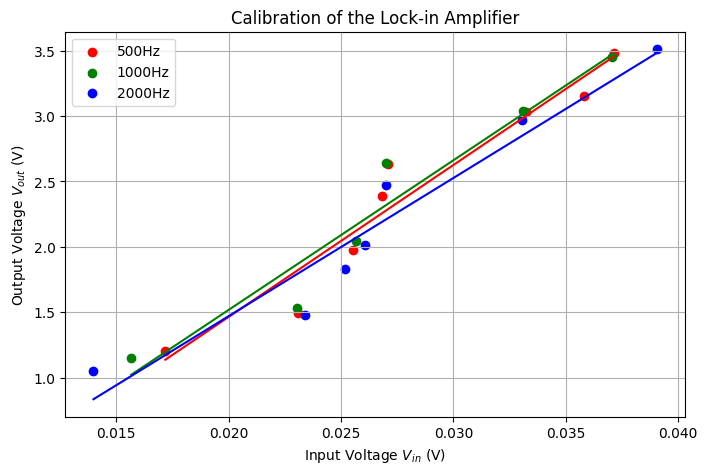
\includegraphics[width=\columnwidth]{Images/CAL_plot.png}
    \caption{Calibration curve of the Lock in amplifier}
    \label{CAL_plot}
\end{figure}

%%%%%%%%%%%%%%%%%%%%%%%%%%%%%%%%%%%%%%%%%%%%%%%%%%%%%%%%%%%%%%%%%%%%%%%%%%%%%%
\subsection{Measurement of Low Resistance}
The calculations for the low resistance are done using the formula in \ref{LR_eqn}. The results are shown in the Table 2 itself. The obtained value of the Low resistance r is:

\begin{equation}
    r=1.075\Omega
\end{equation}

%%%%%%%%%%%%%%%%%%%%%%%%%%%%%%%%%%%%%%%%%%%%%%%%%%%%%%%%%%%%%%%%%%%%%%%%%%%%%%
\subsection{C-V Profiling of Solar Cell}

The data shown in the GitHub Repository are plotted in python and the corresponding plots are made. The linear fitting of the $1/C^2$ vs $V_R$ is done. In this part the CV profiling is done in dark conditions for both of the solar cells. The data are linear fitted and the slopes and intercepts are tabulated in the Table-\ref{CV_slope_table}. The further calculations are as follows. The plots are shown in the Figure-\ref{CV_poly_1} and Figure-\ref{CV_poly_2} for the polycrystalline one and in Figure-\ref{CV_mono_1} and Figure-\ref{CV_mono_2} for the monocrystalline one.


\begin{table}[H]
    \centering
    \resizebox{\columnwidth}{!}{%
    \begin{tabular}{|c|c|c|}
    \hline
    \textbf{Type$->$}                        & \textbf{Monocrystalline} & \textbf{Polycrystalline} \\ \hline
    \textbf{slope,m}                       & 5.743692249              & 53.21159361              \\ \hline
    \textbf{err in slope,$\Delta m$}       & 0.445068424              & 1.604544349              \\ \hline
    \textbf{Intercept $c$}                 & -2.880222429             & -17.33620863             \\ \hline
    \textbf{err in   intercept $\Delta c$} & 0.5725663                & 2.064195013              \\ \hline
    \end{tabular}%
    }
    \caption{Linear fitted parameters for mono and poly crystalline solar cells}
    \label{CV_slope_table}
\end{table}


Let the slope of the $1/C^2$ vs $V$ plot be $m$. Then by equation-\ref{CV_eqn}, the doping density is given by:

\begin{equation}
    \rho = \frac{2}{A^2e\epsilon \epsilon_0 m}
\end{equation}

And the built in potential is given by:
\begin{equation}
    V_{bi} = \frac{c}{m}
\end{equation}

where c is the intercept of the plot.

\begin{figure}[H]
    \centering
    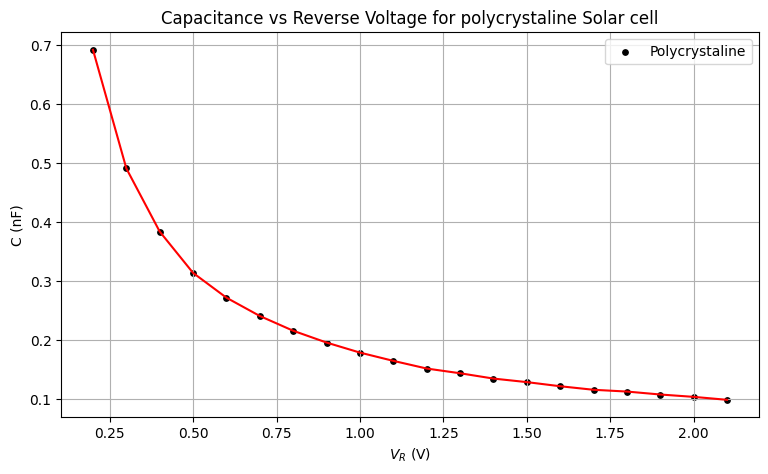
\includegraphics[width=\columnwidth]{Images/CV_poly_1.png}
    \caption{CV Plot for polycrystalline solar cell}
    \label{CV_poly_1}
\end{figure}
So, for the polycrystalline solar cell, using the area as $0.036 m^2$, and the dielectric constant $\epsilon=11.68$ for Silicon, the values are:
\begin{eqnarray}
    \rho^{poly} = 1.753 \times 10^{12} m^{-3} \\
    V_{bi}^{poly} = -0.325 V
\end{eqnarray}

And similarly for the monocrystalline one:
\begin{eqnarray}
    \rho^{mono} = 1.624 \times 10^{15} m^{-3} \\
    V_{bi}^{mono} = -0.501 V
\end{eqnarray}
For the mono crystalline one, $A = 0.0036 m^2$ and the dielectric constant is taken to be 11.68.




\begin{figure}[H]
    \centering
    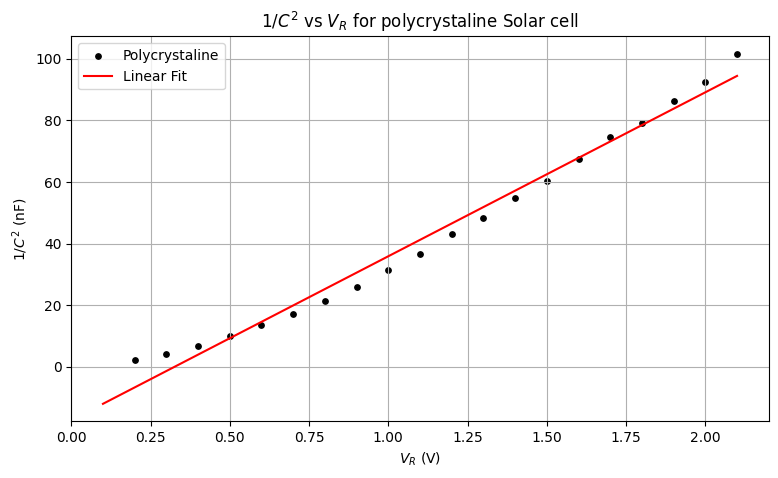
\includegraphics[width=\columnwidth]{Images/CV_poly_2.png}
    \caption{Plot of $1/C^2$ vs $V_R$ for the polycrystalline solar cell}
    \label{CV_poly_2}
\end{figure}



\begin{figure}[H]
    \centering
    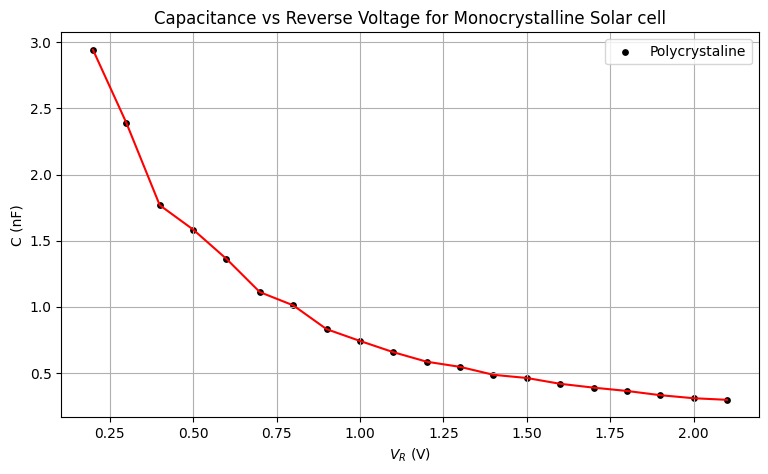
\includegraphics[width=\columnwidth]{Images/CV_mono_1.png}
    \caption{CV Plot for monocrystalline solar cell}
    \label{CV_mono_1}
\end{figure}



\begin{figure}[H]
    \centering
    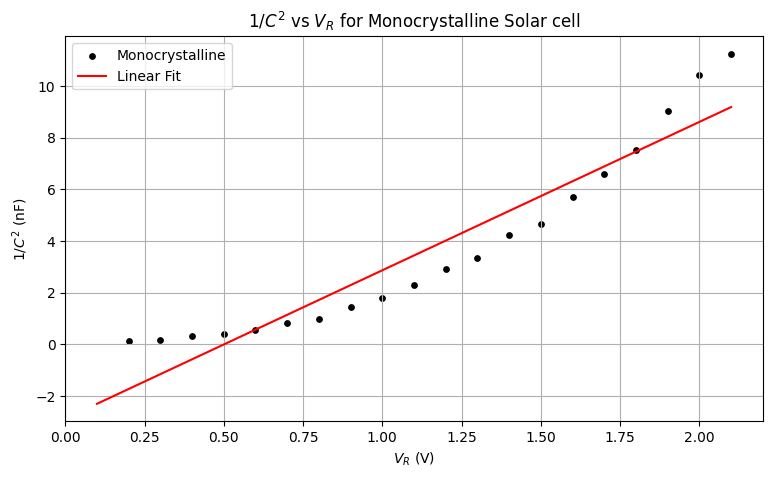
\includegraphics[width=\columnwidth]{Images/CV_mono_2.png}
    \caption{Plot of $1/C^2$ vs $V_R$ for the monocrystalline solar cell}
    \label{CV_mono_2}
\end{figure}

%%%%%%%%%%%%%%%%%%%%%%%%%%%%%%%%%%%%%%%%%%%%%%%%%%%%%%%%%%%%%%%%%%%%%%%%%%%%%
%%%%%%%%%%%%%%%%%%%%%%%%%%%%%%%%%%%%%%%%%%%%%%%%%%%%%%%%%%%%%%%%%%%%%%%%%%%%%
\section{Error Analysis}


Let $\Delta x$ be the error in the quantity $x$. if the error on x depends on some random errors in the quantities $A, B, C . . .$ like $x=A^a B^b C^c$….etc then the error in the quantity $x$ can be calculated as:


\begin{equation}
    \frac{\Delta x}{x} = \sqrt{(a \frac{\Delta A}{A})^2 + (b \frac{\Delta B}{B})^2 + ...}
    \label{errformula}
\end{equation}

%%%%%%%%%%%%%%%%%%%%%%%%%%%%%%%%%%%%%%%%%%%%%%%%%%%%%%%%%%%%%%%%%%%%%%%%%%%%%
\subsection{Error in the Calibration}

The error in the calibration is just the error in the slopes of the calibration curve which were linear fitted. The value of the amplification factor is calculated out to be:
\begin{equation}
    \Delta \alpha = 13.265 
\end{equation}

The error in the Low resistance, as we can see from Table-\ref{LR_data_table}, we use the standard deviation error. So, we get the value of the low resistance r as:
\begin{equation}
    \Delta r = 0.041 \Omega
\end{equation}

%%%%%%%%%%%%%%%%%%%%%%%%%%%%%%%%%%%%%%%%%%%%%%%%%%%%%%%%%%%%%%%%%%%%%%%%%%%%%
\subsection{Error in the Doping density and built in potential}

From the Equation-\ref{CV_eqn}, we can see that the error in the doping density depends on only on the slope of the $1/C^2$ vs V curve, because other parameters are constants and are already known values. So, the percentage error in the doping density will be same as that of the percentage error in slope. So, on calculating the error using linear regression, the final value of the doping density can be written as:
\begin{eqnarray}
    \rho^{mono} = 0.126 \times 10^{15} m^{-3} \\
    \rho^{poly} = 0.052 \times 10^{12} m^{-3}
\end{eqnarray}

Now for the built in potential, we know its value depends on both of the intercept and slope, so, we will be using the equation-\ref{errformula} for the same, so we will get:

\begin{eqnarray}
    \Delta V_{bi}^{mono} = 0.106V \\
    \Delta V_{bi}^{poly} = 0.123V
\end{eqnarray}



%%%%%%%%%%%%%%%%%%%%%%%%%%%%%%%%%%%%%%%%%%%%%%%%%%%%%%%%%%%%%%%%%%%%%%%%%%%%%
%%%%%%%%%%%%%%%%%%%%%%%%%%%%%%%%%%%%%%%%%%%%%%%%%%%%%%%%%%%%%%%%%%%%%%%%%%%%%
\section{Results}
The results obtained from this experiment are as follows.
\begin{equation}
    \alpha  = 112.144 \pm 13.265
\end{equation}
\begin{equation}    
    r=1.075 \pm 0.041 \Omega
\end{equation}
\begin{equation}
    \rho^{mono} = (1.624 \pm 0.126) \times 10^{15} m^{-3}
\end{equation}
\begin{equation}
    \rho^{poly} = (1.753 \pm 0.052) \times 10^{12} m^{-3}
\end{equation}
\begin{equation}
    V_{bi}^{mono} = (-0.501 \pm 0.106) V
\end{equation}
\begin{equation}
    V_{bi}^{poly} = (-0.326 \pm 0.123) V
\end{equation}

\section{Conclusion and Discussions}

\subsection{Conclusions}

Using the SEELab and some low cost IC's and resistors, we were able to build a lock in amplifier. The calibration of the lock in amplifier was done and the amplification factor was calculated. The low resistance was measured and the CV profiling of the solar cells was done. The doping density and the built in potential of the solar cells were calculated. The results are in good agreement with the literature values. The error in the measurements is also calculated and is found to be within acceptable limits.
It is evident from the data and the calculations that this low-cost method of building a lock in amplifier using SEELab along with Python, both which has an open-source library is very efficient and successful. 


\subsection{Discussions}


\begin{enumerate}
    \item It's possible that the circuit's extremely high feedback resistance is the cause of the high DC offset voltages seen with the TL082 IC. A significant voltage drop resulting from the input bias current might be caused by a high feedback resistance. The high input base current of the TL082 IC is 20 nA. The output has a DC offset as a result of this voltage drop. In a network with numerous integrated circuits connected, each one may contribute to the DC offset; as a result, we will obtain a significant offset voltage.
    \item The phase shift in the output signal is due to the fact that the input signal and the reference signal are not in phase. This phase shift is removed by adding the phase shift to the output signal. However this can be avoided by using a phase shifter circuit or triggering of the SEELab. We didn't use the inbuilt triggering since it was not required for the experiments that we did. 
    \item There was also a problem with the SEELab's Sampling as the sampling was not uniform. For Example. Lets consider 20 samples out of 8192 that we took. Let the first sample has a voltage 0.5 and the 20th has a voltage of 0.6. Lets say an intermediate voltage of 0.55 is also collected. The output array will contain 0.5,0.55,0.5,0.55,0.5...0.6. That is the output oscillated between 0.5 and 0.55 for a few samples before reaching the value of 0.6. This is a problem with the SEELab and not with the lock in amplifier. Otherwise the results could have been more accurate.
\end{enumerate}

\subsection{Sources of error}
\begin{enumerate}
    \item Loose connections and stray capacitance in the circuit can cause errors in the measurements.
    \item Setting the sampling of the SEELab to a perfect value.(not over and under sampling)
\end{enumerate}

\subsection{Future Prospects}
\begin{enumerate}
    \item The Lock in amplifier can be modified to obtain live signals by setting proper triggering and phase shifting circuits.
    \item The SEELab can be modified to have a better sampling rate and a better triggering system.
    \item This Lock in amplifier can be used for other experiments such as measurement of Mutual inductance of two coils, measurement of the phase difference between two signals etc.
    \item The lock-in algorithm can be made more computationally efficient by modifying the python code.
\end{enumerate}


\end{multicols}
\bibliographystyle{plain}
\bibliography{bib.bib}


\end{document}